\chapter{Lecture: 16/05/2025}

Consider a game, you have a probability $p$ of winning, and a probability $1-p$ of losing. 

You can bet 1 euro each time, and if you win you gain 1 euro, if you lose you lose 1 euro, if you run out of money you stop playing.
\begin{figure}[H]
    \centering
    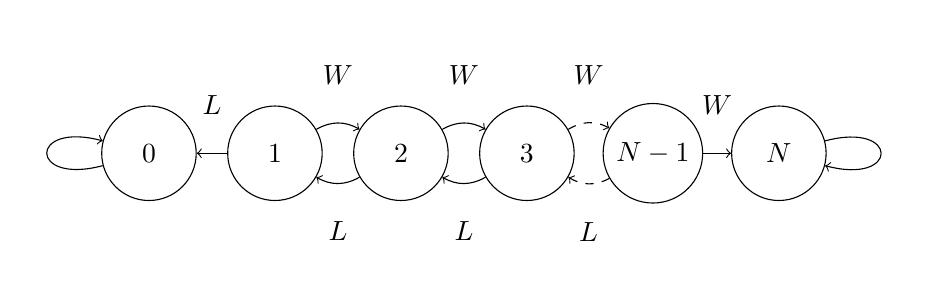
\begin{tikzpicture}[scale=0.8, every node/.style={minimum size=1.2cm}]
        \node[circle,draw] (s1) at (0, 0) {$0$};
        \node[circle,draw] (s2) at (2, 0) {$1$};
        \node[circle,draw] (s3) at (4, 0) {$2$};
        \node[circle,draw] (s4) at (6, 0) {$3$};
        \node[circle,draw] (s5) at (8, 0) {$N-1$};
        \node[circle,draw] (s6) at (10, 0) {$N$};
        \draw[->] (s1) to[loop left] (s1);
        \draw[->] (s2) to node[above] {$L$} (s1);
        \draw[->] (s2) to[bend left=30] node[above] {$W$} (s3);
        \draw[->] (s3) to[bend left=30] node[below] {$L$} (s2);
        \draw[->] (s3) to[bend left=30] node[above] {$W$} (s4);
        \draw[->] (s4) to[bend left=30] node[below] {$L$} (s3);
        \draw[->, dashed] (s4) to[bend left=30] node[above] {$W$} (s5);
        \draw[->, dashed] (s5) to[bend left=30] node[below] {$L$} (s4);
        \draw[->] (s5) to node[above] {$W$} (s6);
        \draw[->] (s6) to[loop right] (s6);
    \end{tikzpicture}
\end{figure}
We can find that $L < W$.

\dots
$$
P(t) = W^t P(0)
$$
\dots
$$
\left(
    \theta^t
\right)_{AB} > 0
$$
\dots

$0$ and $N$ are \bfit{absorbing} states.

We have that a state $\sigma$ is \bfit{transient} if (for $t \gg 1$) $P_\sigma(t) = 0$.

Another important property is the \bfit{ergodicity}: All the states are visited during the process lifetime, and there is no periodicity.

\dots

We can approximate the probability distribution of the transitions as follows:

$$
P_A^{eq} = \dfrac{\#(x(t) = A)}{T}, \qquad P_B^{eq} = \dfrac{\#(x(t) = B)}{T}
$$

Which is \textit{the number of times the process is in state $A$ at time $t$ divided by the total number of transitions $T$} (Same for $B$).

\dots

The \bfit{return time} is the time it takes for a process to return to a given state. For a state $\sigma$, we can define the return time $T_\sigma$ as:
$$
T_\sigma = \min \{t > 0 : x(t) = \sigma | x(0) = \sigma\}
$$

The \bfit{mean return time} $\langle T_\sigma \rangle$ is the average time it takes for the process to return to state $\sigma$ after leaving it. For an ergodic Markov chain, the mean return time is related to the equilibrium probability by:
$$
\langle T_\sigma \rangle = \dfrac{1}{P_\sigma^{\infty}}
$$

This makes intuitive sense: if a state has a high equilibrium probability, it will be visited frequently, leading to a short mean return time. Conversely, states with low equilibrium probabilities will have longer mean return times.

\newpage

All the problems continuous in time but that involves a discrete state space can be solved using a Contionuous Time Markov Chain (CTMC), which are a subset of all the stochastic processes with discrete state space and continuous time.
\vspace{0.4em}
$$
\Pr \big\{x(t) = \sigma\ |\ x(\theta), \quad \theta \in [0, t]\big\}
$$
If we consider an infinitesimal time interval $\dd t$, we can write:
\vspace{0.4em}
$$
\Pr \big\{x(t + \dd t) = \alpha\ |\ x(t) = \sigma\big\}
$$

So the probability of eving more than one transition in the interval is:

$$
\begin{array}{lll}
\Pr \big\{ \ge \text{2 events} & (t, t + \dd t)\big\} & = 0
\\
\Pr \big\{ \text{1 event} & (t, t + \dd t)\big\} & = O(\dd t)
\\
\Pr \big\{ \text{0 events} & (t, t + \dd t)\big\} & = 1 - O(\dd t) \simeq 1
\end{array}
$$

We can define the \bfit{transition rate} as:

$$
\Pr \big\{ x(t + \dd t) = \alpha\ |\ x(t) = \sigma\big\} = W_{\alpha\sigma} \dd t
$$

$W_{\alpha\sigma}$ is always positive and can be $>$ or $<$ than $1$.

\dots

\begin{figure}[H]
    \centering
    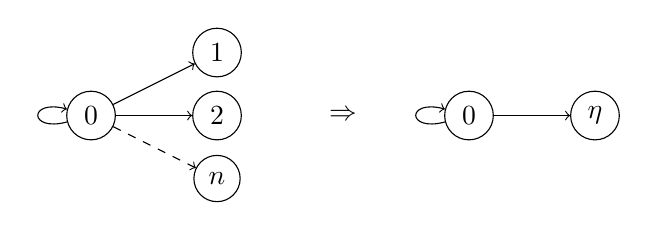
\begin{tikzpicture}[scale=0.8]
        \node[circle,draw] (s1) at (0, 0) {$0$};
        \node[circle,draw] (s2) at (2, 1) {$1$};
        \node[circle,draw] (s3) at (2, 0) {$2$};
        \node[circle,draw] (s4) at (2, -1) {$n$};
        \draw[->] (s1) to[loop left] (s1);
        \draw[->] (s1) to (s2);
        \draw[->] (s1) to (s3);
        \draw[->, dashed] (s1) to (s4);
        \node at (4, 0) {$\Rightarrow$};
        \node[circle,draw] (s1) at (6, 0) {$0$};
        \node[circle,draw] (s2) at (8, 0) {$\eta$};
        \draw[->] (s1) to[loop left] (s1);
        \draw[->] (s1) to (s2);
    \end{tikzpicture}
\end{figure}

To compute the probability of remaining in the state 0, we can collapse all the other states into a single state $\eta$.

\dots

$$
x(t) = \left[ 
    \begin{array}{c}
        S(t)\\
        I(t)
    \end{array}
\right]
$$

With: $(S,I) \to (S-1, I + 1)$,

$$
S(t + \dd t) = S(t) - 1, I(t + \dd t) = I(t) + 1
$$

$$
x(t + \dd t) = x(t) + (-1, 1)
$$

\dots

$$
\begin{cases}
\Pr (Cont) = \Pr \left\{ x(t + \dd t) = x(t) + \left(\begin{smallmatrix}  -1\\[0.2em] 1 \end{smallmatrix} \right) \right\} = \beta \dfrac{I(t)}{N} S(t) \dd t
\\[1em]
\Pr (Rec) = \Pr \left\{ x(t + \dd t) = x(t) + \left(\begin{smallmatrix}  0\\[0.2em] -1 \end{smallmatrix} \right) \right\} = \gamma I(t) \dd t
\end{cases}
\quad \Rightarrow \quad
\begin{cases}
W_{Cont} = \beta \dfrac{I(t)}{N} S(t)\\[0.6em]
W_{Rec} = \gamma I(t)
\end{cases}
$$

\dots

$$
W_{\eta\sigma} = \sum_{\alpha \in \mathcal{S} \setminus \left\{ \sigma \right\}} W_{\alpha\sigma}
$$

\begin{figure}[H]
    \centering
    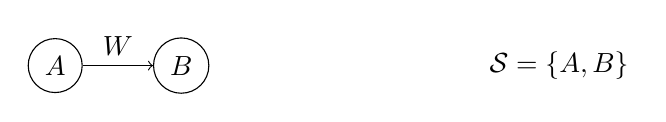
\begin{tikzpicture}[scale=0.8, node distance=1.5cm]
        \node[circle,draw] (s1) at (0, 0) {$A$};
        \node[circle,draw] (s2) at (2, 0) {$B$};
        \draw[->] (s1) to node[above] {$W$} (s2);
        \node at (8, 0) {$\mathcal{S} = \left\{ A, B \right\}$};
    \end{tikzpicture}
\end{figure}
We have that:
$$
\begin{cases}
\Pr \left\{ x(t + \dd t) = B | x(t) = A \right\} = W_{AB} \dd t
\\[0.8em]
\Pr \left\{ x(t + \dd t) = B | x(t) = B \right\} = 1
\end{cases}
$$

$$
P_A(t + \dd t) = (1 - W_{AB} \dd t) P_A(t) \quad \Rightarrow \quad P_A(t + \dd t) = P_A(t) - W P_A(t) \dd t
$$

$$
P_A'(t) = -W P_A(t)
$$

$$
\boxed{P_A(t) = P_A(0) e^{-W t}}
$$

\dots

Let's define $T$ the time of remaining in the state $A$:

\dots

$$
\mathcal P_I(T) = W e^{- W T}
$$

Since this is an exponential distribution, we can compute the mean return time as:

$$
\langle T \rangle = \dfrac{1}{W}
$$

\dots

---

\begin{figure}[H]
    \centering
    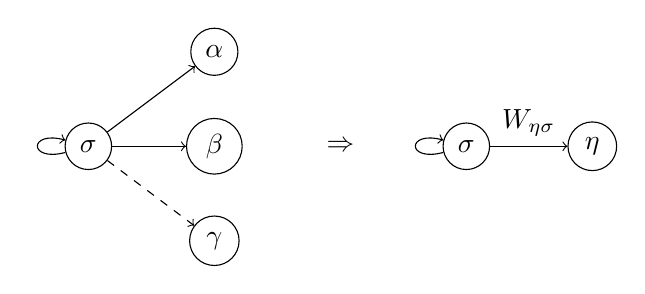
\begin{tikzpicture}[scale=0.8]
        \node[circle,draw] (s1) at (0, 0) {$\sigma$};
        \node[circle,draw] (s2) at (2, 1.5) {$\alpha$};
        \node[circle,draw] (s3) at (2, 0) {$\beta$};
        \node[circle,draw] (s4) at (2, -1.5) {$\gamma$};
        \draw[->] (s1) to[loop left] (s1);
        \draw[->] (s1) to (s2);
        \draw[->] (s1) to (s3);
        \draw[->, dashed] (s1) to (s4);
        \node at (4, 0) {$\Rightarrow$};
        \node[circle,draw] (s1) at (6, 0) {$\sigma$};
        \node[circle,draw] (s2) at (8, 0) {$\eta$};
        \draw[->] (s1) to[loop left] (s1);
        \draw[->] (s1) to node[above] {$W_{\eta\sigma}$} (s2);
    \end{tikzpicture}
\end{figure}

If we want to compute the probability of remaining in the state $\sigma$ for a time $T$, we can write:

$$
P \big\{x(T + \dd t) \in \mathcal S \setminus \{ \sigma \} | x(T) = \sigma \big\}
$$

Also in this case we can collapse the states into a single state $\eta$.

$$
W_{\eta\sigma} = \sum_{\alpha \not = \sigma} W_{\alpha\sigma} = W_{sum}
$$

So we can say that:

$$
\begin{cases}
t_{\eta} \quad x(t_{\eta}) = \sigma
\\
T \sim \exp(\lambda = W_{sum})
\end{cases}
\qquad \Rightarrow \qquad
t_{next} = t_{\eta} + T
$$

$$
\begin{array}{l}
\Pr \{
    x(t_\eta + T + \dd t) = \alpha| x(t + T) = \sigma 
\} = W_{\alpha\sigma} \cdot 1 \cdot \dd t,
\\
\Pr \{
    x(t_\eta + T + \dd t) = \beta| x(t + T) = \sigma 
\} = W_{\beta\sigma} \cdot 1 \cdot \dd t,
\\
\dots
\end{array}
$$

\dots

\newpage

\begin{figure}[H]
    \centering
    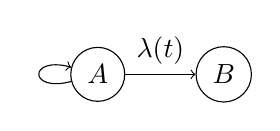
\begin{tikzpicture}[scale=0.8]
        \node[circle,draw] (s1) at (0, 0) {$A$};
        \node[circle,draw] (s2) at (2, 0) {$B$};
        \draw[->] (s1) to[loop left] (s1);
        \draw[->] (s1) to node[above] {$\lambda(t)$} (s2);
    \end{tikzpicture}
\end{figure}

$$
P_A(t + \dd t) = (1 - \lambda(t) \dd t) P_A(t)
$$

$$
P_A'(t) = - \lambda(t) P_A(t) = P_A(t) = P_A(0) e^{-L (t)},
\qquad
L(t) = \int_0^t \lambda(s) \dd s
$$

$$
\mathcal P(T) = \lambda (T) e^{-L(t)}
$$

$$
T  \sim \mathcal P(T)  = \lambda (T) e^{-L(t)}
$$

$$
P(\sigma \to \alpha) = \dfrac{\lambda_{\sigma}(T)}{L_{sum}(t)}
$$

---



\begin{figure}[H]
    \centering
    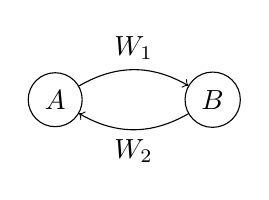
\begin{tikzpicture}
        \node[circle,draw] (s1) at (0, 0) {$A$};
        \node[circle,draw] (s2) at (2, 0) {$B$};
        \draw[->] (s1) to[bend left=30] node[above] {$W_1$} (s2);
        \draw[->] (s2) to[bend left=30] node[below] {$W_2$} (s1);
    \end{tikzpicture}
\end{figure}

$$
\begin{cases}
\dot P_1 (t) = W_2 P_B(t) - W_1 + P_A(t)
\\
\dot P_2(t) = W_1 P_A(t) - W_2 P_B(t)
\end{cases}
\quad \Rightarrow \quad
\begin{array}{l}
    \dot P_A + \dot P_B = 0
    \\
    P_A + P_B = 1
\end{array}
$$

$$
\begin{cases}
\dot P_A = \sum (W_{Ay} P_y - W_{yA}P_A)
\\
\sum_{A \in \mathcal S} P_A(t) = 1
\end{cases}
$$

And we have that:

$$
\dot P_A = - W_1 P_A + W_2 (1 - P_A) = W_2 - (W_1 + W_2) P_A
$$

So, for an equilibrium we have that:

$$
0 = W_2 - (W_1 + W_2) P_A^{eq}
$$

$$
P_A^{eq} = \dfrac{W_2}{W_1 + W_2},
\qquad \qquad
P_B^{eq} = \dfrac{W_1}{W_1 + W_2}
$$

We can write our transition matrix:

$$ W =
\left[
\begin{array}{cc}
 - W_1 & W_2
\\
W_1 & - W_2
\end{array}
\right]
$$

Which is singular, so one of the eigenvalue is $0$.

\dots

$$
\begin{cases}
\dot P_\sigma = \sum (W_{\sigma y} P_y - W_{y\sigma} P_\sigma)
\\
\dot{\underline{P}} = A \underline{P}
\\
\sum_\sigma \dot P_\sigma (t) = 0
\end{cases}
$$

$$
0 = A p^{eq}
$$

\dots

\begin{figure}[H]
    \centering
    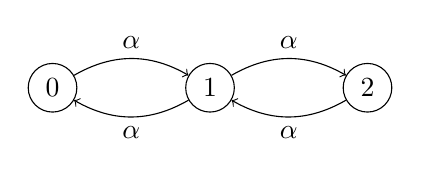
\begin{tikzpicture}
        \node[circle,draw] (s1) at (0, 0) {$0$};
        \node[circle,draw] (s2) at (2, 0) {$1$};
        \node[circle,draw] (s3) at (4, 0) {$2$};
        \draw[->] (s1) to[bend left=30] node[above] {$\alpha$} (s2);
        \draw[->] (s2) to[bend left=30] node[below] {$\alpha$} (s1);
        \draw[->] (s2) to[bend left=30] node[above] {$\alpha$} (s3);
        \draw[->] (s3) to[bend left=30] node[below] {$\alpha$} (s2);
    \end{tikzpicture}
\end{figure}

The steady state is given by:

$$
\begin{array}{llll}
\dot P_0 = & - \alpha P_0 & + \alpha P_1 &
\\[0.5em]
\dot P_1 = & \alpha P_0 & - 2\alpha P_1 + & \alpha P_2
\\[0.5em]
\dot P_2 = &  & \alpha P_1 - & \alpha P_2
\end{array}
$$

\dots

$$
3\phi = 1 \quad \Rightarrow \quad  
\boxed{\phi = \dfrac 13}
$$

we can now generalize this to a system with $N$ states:

\begin{figure}[H]
    \centering
    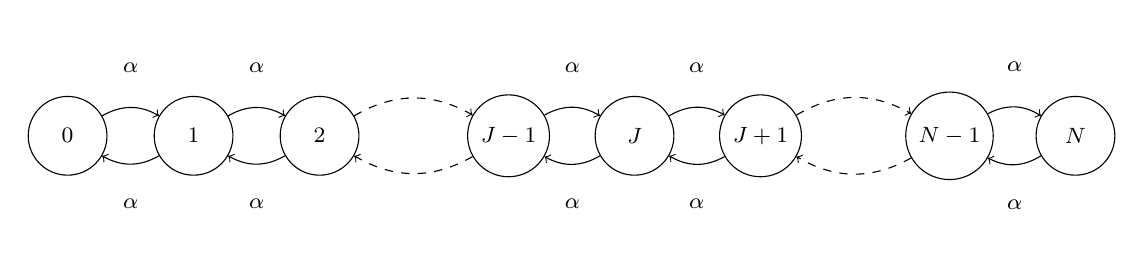
\begin{tikzpicture}[scale=0.8, every node/.style={minimum size=1cm, font=\footnotesize}]
        % Main states
        \node[circle,draw] (s1) at (0, 0) {$0$};
        \node[circle,draw] (s2) at (2, 0) {$1$};
        \node[circle,draw] (s3) at (4, 0) {$2$};
        \node[circle,draw] (s4) at (7, 0) {$J-1$};
        \node[circle,draw] (s5) at (9, 0) {$J$};
        \node[circle,draw] (s6) at (11, 0) {$J+1$};
        \node[circle,draw] (s7) at (14, 0) {$N-1$};
        \node[circle,draw] (s8) at (16, 0) {$N$};
        
        % Transitions with consistent spacing and styling
        \foreach \i/\j in {1/2, 2/3, 4/5, 5/6, 7/8} {
            \draw[->] (s\i) to[bend left=30] node[above] {$\alpha$} (s\j);
            \draw[->] (s\j) to[bend left=30] node[below] {$\alpha$} (s\i);
        }
        
        % Dashed transitions for intermediate states
        \draw[->, dashed] (s3) to[bend left=30] (s4);
        \draw[->, dashed] (s4) to[bend left=30] (s3);
        \draw[->, dashed] (s6) to[bend left=30] (s7);
        \draw[->, dashed] (s7) to[bend left=30] (s6);
    \end{tikzpicture}
\end{figure}

\dots

Let's consider an unidirectional chain, with a single transition rate $\lambda$:

\begin{figure}[H]
    \centering
    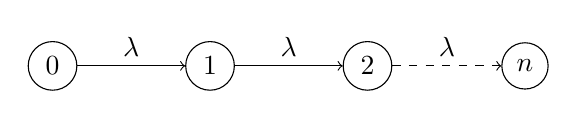
\begin{tikzpicture}
        \node[circle,draw] (s1) at (0, 0) {$0$};
        \node[circle,draw] (s2) at (2, 0) {$1$};
        \node[circle,draw] (s3) at (4, 0) {$2$};
        \node[circle,draw] (s4) at (6, 0) {$n$};
        \draw[->] (s1) to node[above] {$\lambda$} (s2);
        \draw[->] (s2) to node[above] {$\lambda$} (s3);
        \draw[->, dashed] (s3) to node[above] {$\lambda$} (s4);
    \end{tikzpicture}
\end{figure}

$$
\begin{array}{lll}
\dot P_0 = - \lambda P_0\\
\dot P_1 = \lambda P_0 - \lambda P_1\\
\dots\\
\dot P_\sigma = \lambda P_{\sigma} - \lambda P_{\sigma - 1}
\end{array}
$$

\dots

The probability distribution $P_n(t) = \Pr\{N(t) = n\}$ has a simmetry property:

$$
P_n(t) = \dfrac{(\lambda t)^n}{n!} e^{-\lambda t}
$$



